\documentclass{article}
\usepackage{graphicx}
\usepackage[boxruled,linesnumbered]{algorithm2e} 
\usepackage[
top    = 2.5cm,
bottom = 2.5cm,
left   = 3.50cm,
right  = 2.50cm]{geometry}

\begin{document}
\title{LonestarGPU Benchmarks}
\date{}
\maketitle


Lonestar is a collection of real world applications which shows irregular behavior. Irregular in the sense that it contains irregular data structures like graph, tree, priority queues. Many applications like N-body simulation, social networks, data mining, system modelling, compilers and many contains irregular data structures. These applications are more difficult to parallelise. \\

From the compiler point of view, control flow and memory access are very much data dependent. We can not statically predict the behavior of program because input data values determine the runtime behavior of the program.\\

LonestarGPU benchmarks are the implementation of these irregular applications in CUDA. \\

It contains following list of applications -

\begin{itemize}
\item Breadth First Search 
\item Single Source Shortest Path 
\item Minimum Spanning Tree 
\item Barnes Hut N-Body Simulation 
\item Survey Propagation 
\item Delaunay Mesh Refinement 
\end{itemize}


%%%%%%%%%%%%%%%%%%%%%%%%%%%%%%%%%%%%%%%%%%%%%%%%%%%%%%%%%%%%%%%%%%%%%%%%%%%%%%%%%
%%%%%%%%%%%%%%%%%%%%%%%%%%%%%%%%%%%%%%%%%%%%%%%%%%%%%%%%%%%%%%%%%%%%%%%%%%%%%%%%


\section{Breadth First Search (BFS)}
\subsection{Introduction} 

Consider a graph $G = (V, E)$ with a set V which contains n vertices and a set E which contains m directed edges. Given a source vertex s, goal is to traverse the nodes of graph G in breadth first order starting at s. Each newly discovered vertex v, it will update its distance d from s and the predecessor vertex p on the shortest path to s. The pair (u, v) indicates a directed edge in the graph from u to v, and the adjacency list $A = \{ v | (u, v) \epsilon E \}$ is the set of neighboring vertices incident on vertex u. We will replace each undirected edge by two directed edge containing both (u, v) and (v, u). \\


This algorithm measures Graph size and traversal rates in terms of number of directed edges presented in the graph. We have represented graph using adjacency matrix. We have used a compressed sparse row (CSR) sparse matrix format to store the graph in memory which contains two arrays R and C. R is an offset array which contains n+1 entries. Each entry i in R represent address of first neighbor of vertex i in C. C is an array which contains collection of adjacency list of neighbors. We have not done any preprocessing on graphs before storing in CSR format.   \\


\IncMargin{1em}
\begin{algorithm}
	\SetKwData{offset}{offset}
	\SetKwFunction{Push}{Push}\SetKwFunction{Pop}{Pop}
	\SetKwInOut{Input}{input}\SetKwInOut{Output}{output}
	\Input{Vertex set $V$, row offset $R$, column indices $C$, source vertex $s$}
	\Output{Array $dist[]$ with $dist[i]$ containing distance from $s$ to $i$}
	\BlankLine
	\emph{$Q = \{\}$  }\;
	\BlankLine
	\For{$i$ in $V$}{
	\emph{ $dist[i] \leftarrow \infty$ }\;
	}
	\BlankLine
	\emph{ $dist[s] \leftarrow 0$ }\;
	\emph{ $Q\cdot$\Push{$s$} }\;
	\BlankLine
	\While{$Q \neq \{\}$}{
	\emph{ $i = Q\cdot$\Pop{} }\;
		\For{\offset in  $R[i] \dots R[i+1]-1$}{
		\emph{ $j = C[$ \offset$]$}\;
			\If{$dist[j] == \infty$}{
			\emph{ $dist[j] = dist[i] + 1$}\;
			\emph{ $Q\cdot$\Push{}}\;
			} 
		}
	}
\caption{A simple serial BFS algorithm for marking vertex distances from source}\label{algo:Seq_BFS}
\end{algorithm}\DecMargin{1em}


Algorithm \ref{algo:Seq_BFS} is the standard sequential algorithm for BFS, which uses a queue for circulating the vertices. This algorithm visits each vertices and edges exactly once, so it takes O(m + n) time.

%%----------------------------------------------------------------------------


\subsection{ Data Structure used }

LonestarGPU have used \textbf{CSR (Compressed Sparse Row)} format to store graph information and \textbf{Worklist} to store the vertices which will be accessed in perticular iteration. \\

\begin{enumerate}
\item \textbf{ CSR } \hfill \\
\begin{itemize}
\item Compressed Sparse Row (CSR) sparse matrix format is useful to store graph. \\

\begin{figure}
   \centering
   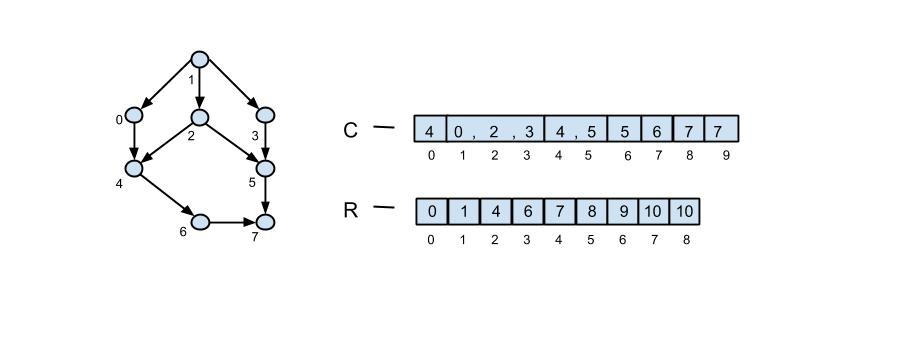
\includegraphics[width=7.0in]{CSR}
   \caption{Sparse Graph Example and It's CSR representation}
   \label{fig:CSR}
\end{figure}


\item It contains two arrays R and C. R is an offset array which contains n+1 entries. Each entry i in R represent address of first neighbor of vertex i in C. C is an array which contains collection of adjacency list of neighbors. \\
\end{itemize}

\item \textbf{ Worklist } \hfill \\

\begin{itemize}
\item It handles atomic read-modify-write operations. It helps in coordinating dynamic placement of data into shared data structures and for maintaing status updates. \\
\item Prefix sum is a suitable approach for data placement. It is a bulk synchronous primitive which can be used to compute scatter address offset for concurrent threads given their dynamic placement requirements. \\
\item If we have a allocation requirement for each thread then prefix sum can be used to calculate the offset address for that thread to start writing in output array. \\
\item In Figure \ref{fig:Prefix_Sum}, prefix sum computes the scatter offset required by each thread to write its vertex to output array. Thread 0 requires 1 space and it's offset is 0 in output array. So thread 0 will stores it's vertices to 0 location in output array. Similarly for other 3 threads. In the output array input order will be preserved. \\

\begin{figure}
   \centering
   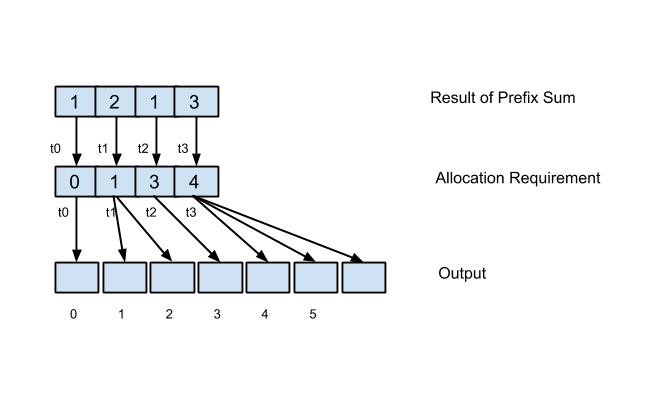
\includegraphics[width=5.0in]{Prefix_Sum}
   \caption{Example of Prefix sum for calculating scatter offsets, Input order is preserved}
   \label{fig:Prefix_Sum}
\end{figure}


\item Worklist Contains following functions :

\begin{itemize}
\item \textbf{Push} : Atomically push a vertex to worklist to its current index.
\item  \textbf{Pop} : Atomically returns the current index vertex and decrements index by 1.
\item  \textbf{display\_items} : Will display all the vertices present in worklist.
\item \textbf{push\_1item} : After performing ProcessEdge, all mark bit information will be returned. To         put all valid mark bit vertices in output worklist in parallel, this function performs this                   operation. This function does prefix sum on mark bit info and computes scatter offset address       in output worklist.
\item \textbf{Pop\_id} : It takes array location as an parameter and returns vertex id. If array location is out of     bound or invalid vertex id, it return -1. All of this is done atomically.
\end{itemize}



\end{itemize}

\textbf{(Cub library is used to perform atomic store and load operations on shared data)}


\end{enumerate}



%%----------------------------------------------------------------------------

\subsection{Parallel BFS}
In above algorithm, it uses queue so it has to label vertices in increasing order of depth. Before going to the next depth, it explores the current depth vertices. So in parallel implementation of BFS it takes advantage of this, where it uses a level synchronous algorithm. This algorithm preserves the sequential ordering while processing each level in parallel. In this case a race condition may occur when multiple threads concurrently discover the vertex v. But there is no harm because all the threads will update the distance of vertex v from s to the same value, which is valid.

\subsubsection{Algorithm Flow}
\begin{enumerate}
\item Initialize all vertices distance from source vertex to infinity.
\item Push source vertex to Input queue.
\item Check all the neigbhors of vertices from Input Queue. If distance of neighbor is infinity then push that neighbor to Output queue.
\item Copy all the vertices from output queue to input queue.
\item Empty the output queue.
\item Repeat steps 3,4,5 until input queue is empty.
\end{enumerate}

%%----------------------------------------------------------------------------

\subsection{CUDA Implementation}

\begin{itemize}
\item LonestarGPU BFS is a implementation of parallel bfs algorithm.
\item It is a work efficient parallel algorithm which performs O(m + n) work. 
\item This implementation uses \textbf{Vertex and Edge Frontier} which is collection of vertices and edges in perticular iteration.
\item To achieve this, in each iteration it examines only the edges and vertices from that iteration's edge and vertex frontier.
\item This implementation prefers to manage vertex frontier out of core, because size of average vertex frontier is small because average out-degree of vertices is small. 
\item While checking for the distance of neighbor, it uses lock to avoid data races.
\item While pushing neighbors to output vertex frontier in parallel, it uses lock to find the correct offset for each block.    
\end{itemize}


 
\IncMargin{1em}
\begin{algorithm}
	\SetKwData{offset}{offset}
	\SetKwFunction{Push}{Push}
	\SetKwInOut{Input}{input}\SetKwInOut{Output}{output}
	\Input{Vertex set $V$, row offset $R$, column indices $C$, source vertex $s$, queues}
	\Output{Array $dist[]$ with $dist[i]$ containing distance from $s$ to $i$}
	\BlankLine 
    \textbf{cilk\_}\For{$i$ in $V$}{
	\emph{ $dist[i] = \infty$ }\;
	}
	\BlankLine
	\emph{\textbf{reducer\_list} input, output}\;
	\emph{$dist[s] = 0$  }\;
    \emph{$iteration = 0$  }\;
    	\emph{$input\cdot$\Push{$s$}}\;
	
	\BlankLine
	\While{$input \neq \{\}$}{
		\emph{ $output =$ \{\} }\;
		\textbf{cilk\_}\For{$i$ in $input$}{
			\For{\offset in  $R[i] \dots R[i+1]-1$}{
			\emph{ $j = C[$ \offset$]$}\;
			\emph{\textbf{Lock} $j$}\;
				\If{$dist[j] == \infty$}{
				\emph{ $dist[j] = iteration + 1$}\;
				\emph{ $output\cdot$\Push{}}\;
				} 
			\emph{\textbf{Release} $j$}\;	
			}
		}
		\emph{ $iteration++$ }\;
		\emph{ $input = output$ }\;
	}
\caption{Cilk Plus parallel BFS constructed using Cilk Plus Reducers }\label{algo:Par_BFS}
\end{algorithm}\DecMargin{1em}


%%----------------------------------------------------------------------------


\subsection{Cilk Plus Implementation}

Algorithm is same as used in CUDA implementation. Instead of \textbf{Worklist}, we have used \textbf{Cilk Plus Reducers} in this implementation. For performing each iteration \textbf{cilk\_for} is used, which will help in dividing task across the workers. At some places where algorithm is performing similar operations across the array, we have used combination of array notations and vectorization. \\ 

\subsubsection{Reducers in place of worklist} 

\begin{itemize}
\item Basic motivation behind using \textbf{Worklist} is, it handles atomic read-modify-write operations. It helps in dynamic placement of data into shared data structures and maintaining status updates. It also preserves the input order. So \textbf{LonestarGPU} implementation uses locks, prefix sum to take care of all the things mentioned above. \\
\item \textbf{Cilk plus Reducers} addresses the problem of computing a value by updating a shared variable in parallel program without data races on that variable. Multiple strands can use Reducers safely in parallel. The runtime makes sure that each strand is using a local copy of reducers which removes the possibility of data races. At the time of synchronization reducer instances are merged into single variable. \\
\item In this implementation, we have used \textbf{List Reducer} to replace the \textbf{Worklist}. Whenever it discovers a new vertex to add in \textbf{Ouput Vertex Frontier}, that strand will add that vertex to \textbf{List Reducer}. There is no need of explicit prefix sum and lock management. Also in discovery of vertices in \textbf{Output Vertex Frontier}, the order of vertices added is not important because in any case it has to examine all vertices in next iteration. \\
\end{itemize}

\subsubsection{Steps and details of implementation in Cilk Plus (Line numbers are mentioned for each step from Algorithm \ref{algo:Par_BFS}) } 


\begin{enumerate}

\item \textbf{Initialization (Line 1-7)}
\begin{itemize}
\item Initialize distances of all the vertices from source vertex to infinity.\\
\item We have used array notations and vectorization to initialize the distances. \\
\item Add \textbf{source} vertex to \textbf{Input Vertex Frontier}. \\
\end{itemize}


\item \textbf{Neighbor\_Gathering (Line 9-20)}
\begin{itemize}
\item Increment \textbf{Iteration}. \\
\item It processes all the vertices from \textbf{Input Vertex Frontier} and gathers their neighbor in parallel.\\
\item It uses \textbf{Cilk\_for} to divide the tasks in multiple workers. \\
\item In \textbf{Cilk\_for} loop, each iteration will have the local variables to store the information of neighbors gathered. \\
\item Create a \textbf{ Cilk Plus Reducer List} to store the valid neighbors for the next iteration.\\
\item Pass all the neighbors to (\textbf{Process\_Edge}).\\
\end{itemize}

\item \textbf{Process\_Edge (Line 12-18)}
\begin{itemize}
\item It validates the neighbor passed. It will check whether the neighbor should be included in next iteration or not.\\
\item We need to use lock here because multiple strands may discover the same vertex as valid vertex and update it's distance. As explained earlier, data race does not affect the correctness of distance but it may push same vertex to \textbf{Cilk Plus List Reducer} multiple times. To avoid duplication, we need to use lock while performing the validation. \\
\item Multiple strands will process neighbors collected in \textbf{Neighbor\_Gathering} process in parallel. \\
\item Each strand will \textbf{lock} the neighbor : \\
\begin{itemize}
\item \textbf{If} distance from source is infinity then push it to the \textbf{Cilk Plus Reducer List}. Set it's distance from the source equal to iteration number. \\
\item \textbf{Else} Do not process that neighbor.  \\
\end{itemize}
\item Release the \textbf{lock}.\\
\end{itemize}

\item \textbf{Swap\_Frontiers (Line 22)} \\
\begin{itemize}
\item Copy all the vertices from \textbf{Cilk Plus Reducer List} to \textbf{Input Vertex Frontier}.\\
\item Make \textbf{Cilk Plus Reducer List} empty. \\
\end{itemize}

\item \textbf{Repeat 2,3,4 until \textbf{Input Vertex Frontier} is empty. (Line 8)} \\

\end{enumerate}


%%%%%%%%%%%%%%%%%%%%%%%%%%%%%%%%%%%%%%%%%%%%%%%%%%%%%%%%%%%%%%%%%%%%%%%%%%%%%%%%%%
%%%%%%%%%%%%%%%%%%%%%%%%%%%%%%%%%%%%%%%%%%%%%%%%%%%%%%%%%%%%%%%%%%%%%%%%%%%%%%%%



\section{Single Source Shortest Path (SSSP)}
\subsection{Introduction}

This benchmark computes the shortest path from a source node to all nodes in a directed graph with non-negative weights. It is based on the principle of relaxation. It replaces optimization to the correct distance gradually by more accurate distance until it reaches to the optimum point. \\

Consider a graph $G = (V, E)$ with a set V containing n vertices and a set E containing m directed edges. The pair (u, v) indicates a directed edge in the graph from u to v, and the adjacency list $A = \{ v | (u, v) \epsilon E \}$ is the set of neighboring vertices incident on vertex u. We have replaced each undirected edge by two directed edge containing both (u, v) and (v, u). For all edged (u, v), compare it's old distance from source with the new distance computed via u and update the distance of v with the minimum value. We need to do this relaxation $|V| - 1$ times. So this algorithm takes $O(|V| * |E|)$. Algorithm \ref{algo:Seq_SSSP} describes the overall workflow. \\

%-------------------------------------------------------------------------------

\IncMargin{1em}
\begin{algorithm}
	\SetKwInOut{Input}{input}\SetKwInOut{Output}{output}
	\Input{Vertex set $V$, Edge set $E$}
	\Output{Array $dist[]$ with $dist[i]$ containing shortest distance from $s$ to $i$, Array $predecessor[]$ with $predecessor[i]$ containing parent vertex of $i$ in shortes path form $s$ to $i$}
	
	\BlankLine
	\For{$i$ in $v$}{
	          \emph{$dist[v] =  \infty $}\;
	          \emph{$predecessor[v] = null$} \;
	}
	\emph{$dist[s] =  0$}\;
	\BlankLine
	\For{$i$ from 1 to $|v| - 1$}{
	     \For{each edge (u, v)}{
	          \If{$dist[u] + wt(u, v) < dist[v]$}{
	                  \emph{$dist[v] = dist[u] + wt(u,v) $}\;    
	                  \emph{$predecessor[v] = u$}\;
	          }
	     }
	}
\caption{A serial version of Bellman Ford Algorithm for graph having non-negative Edges}\label{algo:Seq_SSSP}
\end{algorithm}\DecMargin{1em}


%-------------------------------------------------------------------------------


\subsection{Parallel SSSP} 

This is modified version of \textbf{Bellman Ford Algorithm}, which is similar to the BFS algorithm. The only difference is in validation checking of edge (u, v), where we do not need to check it for all the edges in each iteration. \\

Modification in Bellman Ford algorithm makes it similar to BFS algorithm. In Bellman Ford algorithm, it relaxes all the edges in graph in each iteration for $|v| - 1$ iterations. Each time it checks the current distance with alternative distance and then update the distance array, but there is no need to relax all the edges in each iteration. If vertex v has a distance value that has not ch anged since last time the edges out of v were relaxed, then there is no need to relax the edges out of v second time. So it pushes only those vertices in output vertex frontier whose distance has been updated, which makes it similar to \textbf{Parallel BFS}. This modification helps in parallelization. \\


\subsubsection{Algorithm Flow}
\begin{enumerate}
\item Initialize all vertices distance from source vertex to \textbf{infinity}.
\item Push source vertex to \textbf{input queue}.
\item Check all the neigbhors of vertices from \textbf{input Queue}. Let for edge \textbf{(u,v)}, \textbf{u} is vertex from input queue and \textbf{v} is it's neighbor. 
\begin{itemize}
\item \textbf{If} old distance of v is greater than it's distance via u then push that neighbor to \textbf{output queue}.
\item \textbf{Else} Do not push that neighbor.
\end{itemize} 
\item Copy all the vertices from \textbf{output queue} to \textbf{input queue}.
\item Empty the \textbf{output queue}.
\item Repeat steps 3,4,5 until input queue is empty.
\end{enumerate}

%-------------------------------------------------------------------------------

\subsection{CUDA Implementation}

\begin{itemize}
\item LonestarGPU has implemented this algorithm in CUDA.
\item This implementation uses \textbf{Vertex and Edge Frontier} which is collection of vertices and edges in perticular iteration.
\item It examines only the edges and vertices from that iteration's Edge and Vertex Frontier in each iteration.
\item This implementation prefers to manage vertex frontier out of core, because size of average vertex frontier is small by factor d (average out-degree).   
\item While checking for the distance of neighbor, it uses lock to avoid data races.
\item While pushing neighbors to output vertex frontier in parallel, it uses lock to find the correct offset for each block.    
\end{itemize}

%-------------------------------------------------------------------------------


\IncMargin{1em}
\begin{algorithm}
	\SetKwData{offset}{offset}
	\SetKwFunction{Push}{Push}
	\SetKwInOut{Input}{input}\SetKwInOut{Output}{output}
	\Input{Vertex set $V$, row offset $R$, column indices $C$, source vertex $s$, queues}
	\Output{Array $dist[]$ with $dist[i]$ containing shortest distance from $s$ to $i$}
	\BlankLine 
    \textbf{cilk\_}\For{$i$ in $V$}{
	\emph{ $dist[i] = \infty$ }\;
	}
	\BlankLine
	\emph{\textbf{reducer\_list} input,output }\;
	\emph{$dist[s] = 0$  }\;
    \emph{$iteration = 0$  }\;
    	\emph{$input = \{\}$}\;
    	\emph{$input\cdot$\Push{$s$}}\;
	
	\BlankLine
	\While{$input \neq \{\}$}{
		\emph{ $output =$ \{\} }\;
		\textbf{cilk\_}\For{$i$ in $input$}{
			\For{\offset in  $R[i] \dots R[i+1]-1$}{
			\emph{ $j = C[$ \offset$]$}\;
			\emph{\textbf{Lock} $j$}\;
				\If{$dist[j] + wt(i, j) < dist[i]$}{
				\emph{ $dist[j] = dist[i] + wt(i,j)$}\;
				\emph{ $outputQ\cdot$\Push{}}\;
				} 
			\emph{\textbf{Release} $j$}\;	
			}
		}
		\emph{ $iteration++$ }\;
		\emph{ $input = output$ }\;
	}
\caption{ A Cilk Plus implementation of modified Bellman Ford Algorithm}\label{algo:Par_SSSP}
\end{algorithm}\DecMargin{1em}


%-------------------------------------------------------------------------------



%\begin{figure}
%    \centering
%    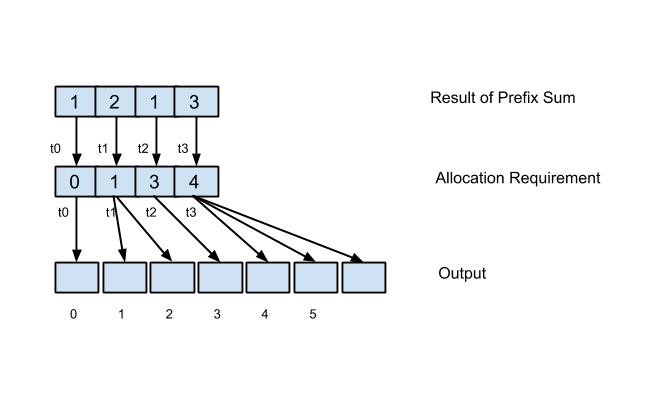
\includegraphics[width=3.0in]{Prefix_Sum}
%    \caption{Simulation Results}
%    \label{simulationfigure}
%\end{figure}

\textbf{ (CSR and Worklist Data Structures are used for storing graph and Vertex Frontier respectively) }


%-------------------------------------------------------------------------------

\subsection{Cilk Plus Implementation}

This algorithm is similar to CUDA implementation. Instead of \textbf{Worklist}, we have used Cilk Plus \textbf{Reducers} in this implementation. For performing each iteration in parallel we have used \textbf{cilk\_for}, which helps in dividing task across the workers. At some places where it is performing similar operations across the array, we have used combination of array notations and vectorization. \\

\subsubsection{Reducers in place of Worklist} 

\begin{itemize}
\item Basic motivation behind using \textbf{Worklist} is, it handles atomic read-modify-write operations. It helps in dynamic placement of data into shared data structures and maintaining status updates. It also preserves the input order. So \textbf{LonestarGPU} implementation uses locks, prefix sum to take care of all the things mentioned above. \\
\item \textbf{Cilk plus Reducers} addresses the problem of computing a value by updating a shared variable in parallel program without data races on that variable. Multiple strands can use Reducers safely in parallel. The runtime makes sure that each strand is using a local copy of reducers which removes the possibility of data races. At the time of synchronization reducer instances are merged into single variable. \\
\item In this implementation, we have used \textbf{List Reducer} to replace the \textbf{Worklist}. Whenever it discovers a new vertex to add in \textbf{Ouput Vertex Frontier}, that strand will add that vertex to \textbf{List Reducer}. There is no need of explicit prefix sum and lock management. Also in discovery of vertices in \textbf{Output Vertex Frontier}, the order of vertices added is not important because in any case it has to examine all vertices in next iteration. \\
\end{itemize}


\subsubsection{Steps and details of implementation in Cilk Plus (Line numbers are mentioned for each step from Algorithm \ref{algo:Par_SSSP})} 

\begin{enumerate}


\item \textbf{Initialization (Line 1-8)}
\begin{itemize}
\item Initialize distances of all the vertices from source vertex to infinity in \textbf{Dist} array.\\
\item We have used array notations and vectorization to initialize the distances in parallel. \\
\item Add source vertex to \textbf{Input Vertex Frontier}. \\
\end{itemize}


\item \textbf{Neighbor\_Gathering (Line 10-22)}
\begin{itemize}
\item Increment \textbf{Iteration}. \\
\item Process all the vertices from \textbf{Input Vertex Frontier} and gather their neighbors in parallel. \\
\item We have used \textbf{Cilk\_for} to divide the tasks across multiple workers. \\
\item In \textbf{Cilk\_for} loop, each iteration will have the local variables to store the information of neighbors gathered. \\
\item Create a \textbf{Reducer List} to store the valid neighbors for the next iteration. \\
\item Pass all the neighbors to (\textbf{Process\_Edge}).  \\
\end{itemize}


\item \textbf{Process\_Edge (Line 13-19)}
\begin{itemize}
\item It checks whether neighbor vertex should be included in next iteration or not. \\
\item We have used \textbf{Lock} here because multiple strands may discover the same vertex as valid vertex and update it’s distance. As explained earlier, data race does not affect the correctness of distance but it may push same vertex to \textbf{Cilk Plus List Reducer} multiple times. To avoid duplication, we need to use lock while performing the validation. \\
\item Multiple strands process edge (u, v) in parallel. Where u is vertex from \textbf{Input Vertex Frontier} and v is neighbor. \\
\item Each strand \textbf{Lock} the neighbor vertex v 
\begin{itemize}
\item Compare it’s old distance from \textbf{Dist} array with alternative distance via it's u. \\
\item \textbf{If} Alternative distance is minimum, it will push the neighbor v to \textbf{Reducer List} and set its distance in \textbf{Dist} array to alternative distance. \\
\item \textbf{Else} Do not process the neighbor v. \\
\end{itemize}
\item Release the \textbf{Lock}.
\end{itemize}

\item \textbf{Swap\_Frontiers (Line 23)} \\
\begin{itemize}
\item Copy all the vertices from \textbf{Cilk Plus Reducer List} to \textbf{Input Vertex Frontier}.\\
\item Make \textbf{Cilk Plus Reducer List} empty. \\
\end{itemize}

\item \textbf{Repeat 2,3,4 until \textbf{Input Vertex Frontier} is empty. (Line 9)} \\


\end{enumerate}

%%%%%%%%%%%%%%%%%%%%%%%%%%%%%%%%%%%%%%%%%%%%%%%%%%%%%%%%%%%%%%%%%%%%%%%%%%%%%%%%%%
%%%%%%%%%%%%%%%%%%%%%%%%%%%%%%%%%%%%%%%%%%%%%%%%%%%%%%%%%%%%%%%%%%%%%%%%%%%%%%%%


\section{Minimum Spanning Tree (MST)}

\subsection{Introduction}

This benchmark uses \textbf{Boruvka's algorithm} to compute the minimum spanning tree in a graph with edges having distinct weights. This algorithm begins with each vertex as a separate component. It finds a edge with minimum weight which connects two different components. After discovery of minimum weight edge, this algorithm merges those two components into one and reduces number of components bye one. It repeats the process until number of components remain same. In the end, the set of edges discovered is a minimum spanning tree.  

%-------------------------------------------------------------------------------
\subsection{Data Structures Used}
Both the implementation uses \textbf{CSR (Compressed Sparse Row)} format to store graph information and \textbf{ComponentSpace} to store the component information.

\begin{itemize}
\item \textbf{ComponentSpace}

\begin{itemize}
\item ComponentSpace uses disjoin set data structure in it. \\
\item Array is used to represent a set, where array value represents representative of that set.
\item ComponentSpace uses \textbf{Union-Find} algorithm with \textbf{Path Compression}. It has two main operations \textbf{Union} and \textbf{Find}.
\begin{itemize}
\item \textbf{Find} - It takes element as an input and determines which set contains that element. It returns the representative of that set.
\item \textbf{Union} - It joins two subsets into one. It replaces the representative of smaller set by representative of bigger set. \\
\end{itemize}
\item \textbf{Path Compression} is an improvement in this algorithm which reduces time required for \textbf{Find} operation from O(n) to O(log n). \\
\item \textbf{ComponentSpace} stores following information -
\begin{itemize}
\item Number of elements
\item Number of components
\item Array to store representative of each element ( Which set it belongs to )
\item Array to store whether a element is representative or not  \\
\end{itemize}
\item As it unifies multiple pair of components in parallel, there is chance that there is common component in more than one pair. So we need \textbf{Locks} for the synchronization.\\ 
\end{itemize}

\end{itemize}

%-------------------------------------------------------------------------------

\subsection{Parallel MST}

This algorithm repeatedly relaxes the minimum weight edges. If we explicitly relaxe the edges, it will modify the graph. To avoid this, this algorithm keeps track of number of components that have been merged. After each iteration number of components reduces and size of component increases. If given graph is connected then this algorithm will terminate when number of components is one. Otherwise it will terminate when number of components remains unchanged after an iteration. \\

\textbf{ Algorithm flow : } 
\begin{itemize}
\item Find minimum weight edge going out of each vertex. \\
\item Find minimum weight edge going out of each component (let's call it Representative) and it's partner to merge. \\
\item Verify that representative and partner is valid. \\
\item Merge verified representative with it's partner component. \\
\item Repeat above steps until number of components remain unchanged. \\
\end{itemize}


%-------------------------------------------------------------------------------

\subsection{CUDA Implementation}

LonestarGPU has implemented this algorithm in CUDA on GPU. This implementation uses \textbf{ComponentSpace} data structure to manage the operations on components. It performs each step mentioned in \textbf{Algorithm flow} in parallel by dividing work across maximum block available on GPU. Every single thread available across the GPU SMs accesses a single element and processes it in parallel. For the synchronization, it uses atomic operations. This version has implemented each step from \textbf{Algorithm Flow} as separate global kernel.  


%-------------------------------------------------------------------------------

\IncMargin{1em}
\begin{algorithm}
	\SetKwData{offset}{offset}
	\SetKwFunction{Push}{Push}
	\SetKwInOut{Input}{input}\SetKwInOut{Output}{output}
	\Input{Vertex set $V$, row offset $R$, column indices $C$}
	\Output{$mst$ containing minimum spaning tree cost}
	
    \emph{$Num\_Comp$ = $|V|$}\;
    \emph{$Old\_Comp = 0$}\;
    \BlankLine
    
    \While{$Old\_Comp \neq Num\_Comp$}{	 
    \emph{$Old\_Comp = Num\_Comp$}\;
    \textbf{cilk\_}\For{$i$ in $V$}{
	      \emph{$Elem\_wt[i] = Comp\_wt[i] = \infty$}\;
	      \emph{$Partner[i] = Comp\_to\_elem[i] = i$}\;
	      \emph{$Process\_in\_next\_itr = false$}\;
	}
	
	\BlankLine
    \textbf{cilk\_}\For{$i$ in $V$}{
        \emph{$src\_comp = Comp\_to\_elem[i]$}\;
	    \For{All edges $(i,v)$ going out of $i$}{
		   \emph{$Elem\_wt[i]$ = min(Old value, weight of $(i,v)$)}\;
	       \emph{$Comp\_wt[src\_comp]$ = min(Old value, weight of $(i,v)$)}\;
	       \If{Old value $>$ weight of (i,v)}{
	           \emph{$dst\_comp = Comp\_to\_elem[v]$}\;
	           \emph{$partner[i] = dst\_comp$}\;
             } 	       
	    }
	}
	
	\BlankLine 
    \textbf{cilk\_}\For{$i$ in $V$}{
          \emph{$src\_comp = Comp\_to\_elem[i]$}\;
          \If{$Elem\_w[i] == Comp\_wt[src\_comp]$}{
              \emph{Mark this node as representetive};\
          }
	}	
	
	\BlankLine 
    \textbf{cilk\_}\For{All Representative Nodes}{
          \If{Representative and Partner values are correct}{
              \emph{$Process\_in\_next\_itr[i] = True$};\
          }
	}
	
	\BlankLine 
    \textbf{cilk\_}\For{$i$ in $Process\_in\_next\_itr$}{
          \emph{\textbf{Lock} $src$ and $dst$ components}\;
          \emph{Merge smaller component into larger component}\;
          \emph{$num\_Comp--$}\;
          \emph{\textbf{Release} lock}\;
	}	
	%}	
}
\caption{ A Cilk Plus implementation of Boruvka's algorithm}\label{algo:Par_MST}
\end{algorithm}\DecMargin{1em}


\subsection{Cilk Plus Implementation}

We have used the same algorithm as CUDA implementation. We have used \textbf{Cilk\_for} to divide work across multiple strands. We have used \textbf{Atomic} operations for the synchronization. To update the weight of minimum spanning tree and number of components after each iteration, we have used \textbf{Cilk Plus reducer\_opadd}. To get the best result, we have tested it using different grain size for all \textbf{Cilk\_for} loops used in this implementaion. In initialization of data, we have used array notations and vectorization. We have used \textbf{Reducer List} to store the representative of components so instead of verifying all nodes, it verifies only representative vertices.     


\subsubsection{Prerequisite}
This implementaion uses following arrays :
\begin{itemize}
\item \textbf{Elem\_wt} - Stores minimum weight edge going out of each vertex.
\item \textbf{Comp\_wt} - Stores minimum weight edge going out of each component.
\item \textbf{Partner} - Stores a valid component for merging.
\item \textbf{Comp\_to\_elem} - Stores a component representative of each vertex.
\item \textbf{Process\_in\_next\_itr} - Stores whether a representative is valid for merging or not.     
\end{itemize}




\subsubsection{Steps and details of Cilk Plus implementation (Line numbers are mentioned for each step from Algorithm \ref{algo:Par_MST})} 
\begin{enumerate}


\item \textbf{Initialization : Line(5-9)}
\begin{itemize}
\item Initialize following arrays with the use of Array Notations and Vectorization :
\begin{itemize}
\item \textbf{Elem\_wt } : Initialize each value to Infinity.
\item \textbf{Comp\_wt} : Initialize each valeue to Infinity.
\item \textbf{Partner} : Initialize each value to itself.
\item \textbf{Comp\_to\_elem} : Initialize each value to itself.
\item \textbf{Process\_in\_next\_itr} : Initialize each value to false. \\
\end{itemize}
\item Initialize \textbf{mst\_weight} to 0. 
\item Initialize \textbf{Num\_of\_components} to number of vertices.
\end{itemize}


\item \textbf{Find\_MinWt\_Comp : Line(10-20)}
\begin{itemize}
\item Divide total number of vertices across multiple workers using \textbf{Cilk\_for} loop. \\
\item For each vertex, find a minimum weight edge (u,v) going out of that vertex which connects to vertex from other component and store it in \textbf{Elem\_wt} array.\\
\item If (u,v) is minimum for the component it belongs to then update \textbf{Comp\_wt} array value for that component by weight of (u,v).\\
\item Also update \textbf{Partner} array with the component of v. \\
\end{itemize}

\item \textbf{Find\_Representative : Line(21-26)}
\begin{itemize}
\item Divide total number of vertices across multiple workers using \textbf{Clik\_for} loop.\\
\item For each vertex, check if it has a minimum weight edge going out of that component and connects to other component. If it is then mark it as a representative of that component.\\
\item This algorithm uses this representative at the time of merging two components.\\
\end{itemize}

\item \textbf{Verify\_Representative : Line(27-31)}
\begin{itemize}
\item Divide all the \textbf{representative} vertices across multiple workers using \textbf{Cilk\_for} loop. \\
\item Verify that \textbf{Partner} array and \textbf{representative} marked are valid values. \\
\item If verified values are correct then update \textbf{Process\_in\_next\_itr} array value for the \textbf{representaive} vertex to \textbf{True} for merging two components. \\
\end{itemize}

\item \textbf{Unify\_Components : Line(32-37)}
\begin{itemize}
\item For each \textbf{Process\_in\_next\_itr} True values, merge it with \textbf{Partner} component. \\
\item At the time of merge, it merges smaller component with the larger one. \\
\item Reduce number of components by 1 and increase \textbf{mst} value by \textbf{Comp\_wt} value. \\
\end{itemize}

\item \textbf{Repeat steps 1,2,3,4,5 until number of components remain unchanged. : Line(3)}
\end{enumerate}


%%%%%%%%%%%%%%%%%%%%%%%%%%%%%%%%%%%%%%%%%%%%%%%%%%%%%%%%%%%%%%%%%%%%%%%%%%%%%%%%%%
%%%%%%%%%%%%%%%%%%%%%%%%%%%%%%%%%%%%%%%%%%%%%%%%%%%%%%%%%%%%%%%%%%%%%%%%%%%%%%%%


\section{Survey Propagation (SP)}

\subsection{Introduction}
Survey Propagation is a heuristic SAT solver based on Bayesian inference. This algorithm uses a bipartite graph which contains clauses on one side and variables on other side. Edges have either +1 if varialbe in the clause has positive value otherwise -1 value. If Variable is not present in clause then there is no edge between that clause and variable. This algorithm iteratively updates each variable. \\

%-------------------------------------------------------------------------------

\subsection{Data Structures Used}
\begin{enumerate}
\item CSRGraph 
\begin{itemize}
\item It uses Compressed Sparse Row (CSR) format to store information about clauses and variables separately. 
\item It also stores information about bias values. 
\item If we remove variables from graph then we have to modify the graph. So to make it easy, each variable has \textbf{marked bit} information in this data structure.\\
\end{itemize}
\item Edge
\begin{itemize}
\item This data structure stores clause, variable and Pi values of each edge using arrays.
\end{itemize}
\end{enumerate}

%-------------------------------------------------------------------------------

\subsection{Parallel SP} 

This algorithm sets a \textbf{Epsilon} value. In each round of this algorithm, first it processes all the variables and clauses and updates the \textbf{Surveys} until all update values are below the \textbf{Epsilon} value. Then it processes all the calculated \textbf{Surveys}, find most biased variables and fix them. It then removes \textbf{fixed} variables from graph. After each round, if there are only trivial \textbf{Surveys} remaining then pass the graph to simple solver else proceed to next round. \\

There are two termination conditions for the algorithm. If one of them is true, algorithm would terminate. The two termination conditions are :
\begin{itemize}
\item When number of variables remaining are very small, pass the graph to simple solver.
\item If algorithm shows no progress after some fix number of iterations then it will give up.\\
\end{itemize}


\subsubsection{Algorithm Flow}

\begin{enumerate}
\item Get the data from input file and build a bipartite graph.
\item Update the \textbf{Surveys} for all the edges
\item \textbf{If} updated values are above \textbf{Epsilon} then repeat step 2.
\item For each variable, if \textbf{bias} is more then threshold bias then fix that variable and remove it from graph.
\item Repeat algorithm until termination condition is true. 
\end{enumerate}

%-------------------------------------------------------------------------------

\subsection{CUDA Implementation}
\begin{itemize}
\item \textbf{LonestarGPU} has implemented this algorithm in CUDA on GPU. In the beginning of the implementation, they copy all the clause, variable and edge data to GPU. 
\item To implement the step 2 from \textbf{Algorithm Flow}, they have divided all the edges across all the allocated threads. 
\item While fixing the variables, it adds variables having bias value above some fixed value to bias list. So it uses atomic operation to calculate the index in bias array.  
\item After updating bias values, they sort the bias values for fast processing in next iteration. As it stores values of variables and their bias in separate arrays, they have used \textbf{CUDA Cub Dual buffer} to store and \textbf{Cub DeviceRadixSort} to sort. 
\item Where sum of all thread information is required, they have used \textbf{Cub Reduce}.
\end{itemize}

%-------------------------------------------------------------------------------
\IncMargin{1em}
\begin{algorithm}
	\SetKwData{offset}{offset}
	\SetKwFunction{Converge}{Converge}
	\SetKwInOut{Input}{input}\SetKwInOut{Output}{output}
	\Input{\textbf{CSRGraph} clauses,vars and \textbf{Edge} edges}
	\Output{Modified Graph}
	
	\BlankLine
    \emph{Store graph information in $clauses$, $vars$ and $edges$}\;
    \emph{$round = 0$}\;
    \BlankLine
    
    \While{$\Converge{}$}{	 
    
    \emph{\textbf{Sort} list of biased values of variables}\;
    \textbf{cilk\_}\For{All variables}{
    \If{it is a biased variables}{ \emph{\textbf{Fix} it}\;}
    }
	\BlankLine
}

\BlankLine
\emph{\Converge{} :}\
\BlankLine
\emph{$max\_eps = 0$}\;
\While{$max\_eps > EPSILON$}{
\textbf{cilk\_}\For{All \textbf{non-fixed} variables v}{
    \For{All clauses C of V}{
        \emph{Calculate $pi$ values}\;
        \emph{Update $Bias$ Values}\;
        \emph{Update $max\_eps$}\;
   }
}
}
\caption{ A Cilk Plus implementation of Survey Propagation Algorithm}\label{algo:Par_SP}
\end{algorithm}\DecMargin{1em}





\subsection{Cilk Plus Implementation}

%\begin{equation}
%    \label{simple_equation}
%    \alpha = \sqrt{ \beta }
%\end{equation}
We have used same algorithm as CUDA implementation. To divide the work  , like calculating pi values and updating bias, in parallel across the workers we have used \textbf{Cilk\_for} loop. To calculate maximum value across the array, we have used \textbf{Cilk Plus reduces\_max}. To make a reduce operation on array, we have used \textbf{Cilk Plus reducer\_opadd}. While fixing the variable, we add variables having bias value above some fixed value in bias array. So to avoid \textbf{locks}, we have used \textbf{Cilk plus reducers list}. 

\subsubsection{Prerequisite}
This implementation uses following data :
\begin{itemize}
\item \textbf{clauses} - It is a \textbf{CSRGraph} data structure. It stores information about the clauses present in graph.
\item \textbf{vars} - It is a \textbf{CSRGraph} data structures. It stores information about variables present in graph.
\item \textbf{edges} - It is a \textbf{Edge} data structure. It stores information about all edges connecting variables and clauses.
\item \textbf{bias\_list} - It is an array which contains list of variables which will get fixed in that round.
\item \textbf{EPSILON} - It a fixed epsilon value.
\end{itemize}

\subsubsection{Steps and details of Cilk Plus Implementation (Line numbers are mentioned for each step from Algorithm \ref{algo:Par_SP})}

\begin{enumerate}

\item \textbf{Initialization : Line(1-2)}
\begin{itemize}
\item Read the input graph file.
\item Store the information in \textbf{clauses, vars} and \textbf{edges}.
\item It does not fix any variable initialy.
\item Initialize \textbf{round} to 0. \\
\end{itemize}

\item \textbf{Converge : Line(12-21)}
\begin{itemize}
\item Calculate pi values of all the edges of the graph in parallel.
\item Update the bias values of all the variables in the graph in parallel.
\item It uses \textbf{cilk\_for} loop to perform above to operations in parallel. It also uses \textbf{reducer\_max} to calculate maximum bias value to compare with \textbf{EPSILON}.
\item It repeats this step until it gets maximum bias value below the \textbf{EPSILON} or it repeats this step some fixed number of iterations.
\end{itemize}

\item \textbf{Build\_List : Line(4)}
\begin{itemize}
\item Sort the bias list of variables to get the most biased variables in less time.
\item We have sorted the pair of variables array and corresponding bias values array using \textbf{cilkpub} library. This library sorts the given array in parallel.
\end{itemize}

\item \textbf{Decimate : Line(5-9)}
\begin{itemize}
\item Get the most biased variables and mark them as fixed variables.
\item We have used \textbf{cilk\_for} loop to mark fixed variables in parallel.
\end{itemize}

\item \textbf{Repeat steps 2,3,4 until it can not \textbf{Converge} modified graph. : Line(3)} \\

\end{enumerate} 

%%%%%%%%%%%%%%%%%%%%%%%%%%%%%%%%%%%%%%%%%%%%%%%%%%%%%%%%%%%%%%%%%%%%%%%%%%%%%%%%%%
%%%%%%%%%%%%%%%%%%%%%%%%%%%%%%%%%%%%%%%%%%%%%%%%%%%%%%%%%%%%%%%%%%%%%%%%%%%%%%%%

\section{Barnes Hut N-Body Simulation}

\subsection{Introduction}
This algortihm simulates the gravitational force acting on galactic cluster. It initializes velocities and positions of the galaxies. This algorithm calculates forces acting on each galaxies and calculates the motion of the galaxies for a number of time steps.

\subsection{Parallel BH}
Parallel BH uses J. Barnes and P. Hut.A hierarchical O(NlogN) force calculation algorithm. Parallelism comes from independent force calculation of each body. This algorithm uses an \textbf{Octree} data structure, which is a hierarchical tree data structure. This data structure is useful to calculate the force that n bodies in the system induce upon each other. To calculate force for n bodies, it takes n\textsuperscript{2} operations to calculate. The Barnes Hut algorithm hierarchically partitions the total volume into smaller cells. In an Octree, each partitioned cell will represent a intermediate node. It will contain combined mass and centre of gravity of all the bodies from the cell it belongs to. All the leaf node are individual bodies present in the system. \\

While calculating force, if body is so far then it calculates force with that cell instead of calculating it with all the bodies from that cell. So this algorithm reduces number of operations from n\textsuperscript{2} to nlogn. It centre of mass is not sufficiently far away then it looks into the all subcells and performs the calculations.    

\subsubsection{Algorithm Flow}
\begin{enumerate}
\item Read input file.
\item Make an Octree.
\item For each body in the system, insert it in Octree.
\item Calculate centre of gravity and combined mass of each cell.
\item For each body in the system, calculate force.
\item According to calculated force, cahnge position and velocities of the bodies.
\item Repeat 2,3,4,5,6 for number of Time steps mentioned.
\end{enumerate}

\subsection{CUDA Implementation}
\begin{itemize}
\item \textbf{LonstarGPU} has implemented this algorithm in CUDA on GPU.
\item They have done warp based execution. It makes sure the all the threads belonging to that warp are executing same instruction. In force calculation kernel they have used warp based execution.
\item To improve the executiion, this algorithm sort the bodies according to their distance.
\item They have implemented \textbf{Wait-free pre-pass}, where a thread which has discoverd the child does not wait for the other threads and start processing the children.
\item For synchronisation, they have used \textbf{\_\_syncthread} and \textbf{\_\_threadfence}. 
\end{itemize}


\subsection{Cilk Plus Implementation}

We have implemented same algorithm as CUDA implementation. We have used \textbf{cilk plus max/min reducers} to calculate the square boundary of the area of all bodies present. To build a octree, all bodies are inserted into the octree in parallel. When more then one body is accessing same intermediate node then we have used a \textbf{lock} there to avoid the data race. Otherwise it will insert multiple bodies in parallel. We have used \textbf{cilk\_for} to divide this work in parallel. 

\subsubsection{Prerequisite}
This implementation uses following data :

\begin{itemize}
\item \textbf{n} - Number of bodies
\item \textbf{pos\_x, pos\_y, pos\_z} - These arrays store x,y,z coordinates of bodies present in the system.
\item \textbf{vel\_x, vel\_y, vel\_z} - These arrays store velocities of bodies in x,y,z direction.
\item \textbf{mass} - This array stores the mass of all the bodies present in the system.
\item \textbf{tree} - This is an array of size 8 * (n + 1). It stores the octree data structure. First n to 2*n locations are reserved to prepresent intemediate node. In octree, if place is empty then it stores -1. If place contains leaf node then it store body. If it is an intermediate node then it contains intermediate node number. Last 8 locations in array represent 8 children of root.  
\end{itemize}


\IncMargin{1em}
\begin{algorithm}
	\SetKwData{offset}{offset}
	\SetKwFunction{Push}{Push}
	\SetKwInOut{Input}{input}\SetKwInOut{Output}{output}
	\Input{mass, velocity and position arrays}
	\Output{Changed values after given number of iterations}
	
    \emph{Generate random input data}\;
    \emph{Initialize $mass$,$vel$ and $pos$ arrays}\;
    \emph{Initialize last 8 locations of $tree$ array with -1 }\;
    \BlankLine
    
    
   \For{Number of timesteps}{    
    
    \emph{\textbf{reducer\_max} max\_x, max\_y, max\_z}\;
    \emph{\textbf{reducer\_min} min\_x, min\_y, min\_z}\;
	\textbf{cilk\_}\For{All values in pos arrays}{
	    \emph{calculate max\_x, max\_y, max\_z from pos\_x, pos\_y, pos\_z}\;
	    \emph{calculate min\_x, min\_y, min\_z from pos\_x, pos\_y, pos\_z}\;
	}    
	\emph{$radius = max(max\_x - min\_x,max\_y - min\_y,max\_z - min\_z)$}\;
    
    \BlankLine
    \textbf{cilk\_}\For{Each body}{
        \emph{Compute \textbf{child} of root where a body should be inserted}\;
        \eIf{\textbf{child} is locked}{
           \emph{Try again for this body later}\;
        }{ \eIf{\textbf{child} contains -1}{
               \emph{Insert body}\;
           }{
               \emph{\textbf{Lock} child}\;
               \emph{Insert old and new body to next level}\;
               \emph{\textbf{Release} child}\;
           }
        }
        
    }    
    
    
    \BlankLine
    \textbf{cilk\_}\For{All intermediate nodes in tree}{
          \eIf{All children of node are ready}{
               \emph{Compute \textbf{centre of mass} and \textbf{centre of gravity}}\;
          }{
               \emph{Wait for all children to get ready}\;
          }         
    }
    
    \BlankLine
    \textbf{cilk\_}\For{All leaf nodes in tree}{
	      \emph{Calculate \textbf{offset} address in \textbf{sort} array}\;
          \emph{Place it to its \textbf{offset} address}\;
	}
	
	\textbf{cilk\_}\For{All the bodies}{
	     \For{All tree nodes}{
	          \eIf{Node is too far from body}{
	               \emph{Compute force using that cell's information}\;
	          }{
	               \emph{Iterate over the individual child of that node to compute the force}\;
	          }
	     }
	}
	
	\textbf{cilk\_}\For{For all Bodies}{
	   \emph{Update pos and vel arrays}\;
	}
	
}	
\caption{ A Cilk Plus implementation of Barnes Hut N-Body Simulation}\label{algo:Par_BH}
\end{algorithm}\DecMargin{1em}



\subsubsection{Steps and details of Cilk Plus Implementation (Line numbers are mentioned for each step from Algorithm \ref{algo:Par_BH})}

\begin{enumerate}

\item \textbf{Initialization : Line(1-3)}
\begin{itemize}
\item Generate a random input data.
\item Initialize \textbf{mass, vel} and \textbf{pos} arrays.
\item Initialize last 8 locations of \textbf{tree} array with -1.
\end{itemize}

\item \textbf{Build\_Box : Line(5-11)}
\begin{itemize}
\item Calculate \textbf{min} and \textbf{max} values from all \textbf{pos} arrays.
\item Calculate the area of the box.
\item It calculate \textbf{max} and \textbf{min} values using \textbf{max/min reducers}.
\end{itemize}

\item \textbf{Build\_Tree : Line(12-25)}
\begin{itemize}
\item This function builds octree for give set of bodies.
\item For each body, it computes the child of a root it should be inserted in. Then it starts traversing from the root. 
\begin{itemize}
\item \textbf{If} child is \textbf{locked} then try again later.
\item \textbf{Else} 
\begin{itemize}
\item \textbf{If} it contains -1, then insert a body at that location.
\item \textbf{Else} : It means that there is another body present at that location. So \textbf{Lock} it and insert old body and new body to next level of tree. While inserting to the next level, it checks all above conditions again.
\end{itemize}
\end{itemize}  
\item We have used \textbf{cilk\_for} to insert bodies in parallel.
\item We have used \textbf{atomic locks} to avoid the data races.
\end{itemize}

\item \textbf{Summarize : Line(26-32)}
\begin{itemize}
\item Compute centre of gravity and centre of mass of all intermediate cells.
\item It starts computing from leftmost intermediate node in the \textbf{tree} array because leftmost \textbf{intermediate} node will have no intermediate node in it. So it can calculate it's centre of gravity and centre of mass.
\item In case, one of the children is not ready then it will wait until it becomes ready.
\end{itemize}

\item \textbf{Sort : Line(33-36)}
\begin{itemize}
\item Sorts body according to \textbf{inorder traversal} of an octree.
\item It calculates offset address in \textbf{sort} array for all \textbf{bodies} present in octree. 
\item Place all bodies to their offset address to make them spatially close.
\item As we are calculating offset address, we have done it in parallel using \textbf{cilk\_for}.  
\end{itemize}

\item \textbf{Compute\_Force : Line(37-45)}
\begin{itemize}
\item Calculates force acting on each body.
\item If body is far away then it coputes force acting on it using cell information. Then there is no need to calculate force from other bodies of that cell.
\item If body is not far then it calculates force acting on it.
\item We have used \textbf{cilk\_for} to divide these calculations in parallel. 
\item \textbf{Sort} function makes this function faster because bodies are spatially close.
\end{itemize}

\item \textbf{Advance : Line(46-48)}
\begin{itemize}
\item Updates the \textbf{pos} and \textbf{vel} arrays using calculated force.
\item This is purely parallel function where we have used vectorization with the \textbf{cilk\_for} loop.
\end{itemize}

\item \textbf{Repeat 2,3,4,5,6 for given number of timesteps. : Line(4)}

\end{enumerate}

%%%%%%%%%%%%%%%%%%%%%%%%%%%%%%%%%%%%%%%%%%%%%%%%%%%%%%%%%%%%%%%%%%%%%%%%%%%%%%%%%%
%%%%%%%%%%%%%%%%%%%%%%%%%%%%%%%%%%%%%%%%%%%%%%%%%%%%%%%%%%%%%%%%%%%%%%%%%%%%%%%%

\section{Delaunay Mesh Refinement (DMR) }

\subsection{Introduction}

This algorithm produces a qaulity Delaunay mesh. Qaulity Delaynay mesh is a Delauney trangulation with additional constraint that no angle of any triangle in a mesh should be less than 30 degrees. This algorithm takes a undefined mesh as an input and produces a mesh satisfying the above constraint. This algorithm fixes badly shaped triangles successively. 


\subsection{Parallel DMR}

This algorithm performs refinement on 2D Delaunay mesh. 2D Delaunay mesh is a set of points having the property that circumcircle of any trianlge in a mesh should not contain any other point from that mesh. If there exist other point in a circumcircle then thet triangle will be marked as bad triangle. This algorithm takes set of all bad triangle and re-triangulate them. This process may affect other good neighborhood triangles, called cavity. So this algorithm iteratively fix this cavity until all the triangles present in the mesh satisfy the given constraint. Parallelism arrise from the set of bad trianlge, which will be re-triangulated.

\subsubsection{Algorithm Flow}
\begin{enumerate}
\item Check whether a bad triangle is present or not.
\item Find the affected triangles in the neighborhood by that bad triangle.
\item Re-triangulate all the triangles in the cavity.
\item Find new bad triangles and process them until there is no bad triangle in the mesh.
\end{enumerate}



\subsection{CUDA Implementation}
\begin{itemize}
\item \textbf{LonestarGPU} has implemented this algorithm in CUDA on GPU.
\item They have used \textbf{Worklist} data structure (Explained in BFS) to store the bad triangles of each iteration.
\item Instead of using locks, they have used barrier based exclusive ownership detection which helps in avoiding conflicts. For this they have used \textbf{CUDA cub library}.
\item They have distributed bad triangles to the threads to avoid the overlapping of cavities.
\end{itemize}


\subsection{Cilk Plus Implementation}
We have implemented this algorithm same as CUDA implementation. We have used \textbf{Reducers list} instead of \textbf{Worklist} to maintain the bad triangle of each iteration. \textbf{Reducers list} helps in managing data races. Also to divide all the bad triangles across workers, we have used \textbf{cilk\_for}. When multiple workers try to access the same cavity, we have used \textbf{locks} to avoid the conflict. 

\subsubsection{Prerequisite}
It uses following data structures :
\begin{itemize}
\item \textbf{Mesh} - This data structure contains information about number of elements, their (x,y) coordinates, whether element is bad or not. It stores all the information in separate arrays.
\end{itemize}

\subsubsection{Steps and details of Cilk Plus implementation}
\begin{enumerate}

\item \textbf{Initialization}
\begin{itemize}
\item Read input file and stores the mesh information in \textbf{Mesh} data structure.
\item Set number of bad triangles to 0.
\item Create a \textbf{Input Reducer List} to store bad triangles.
\end{itemize}

\item \textbf{Check\_Triangles}
\begin{itemize}
\item Check all the triangles from \textbf{Mesh} for the given constraint.
\item \textbf{If} a triangle is bad then push it to the \textbf{Input Reducer list}.
\item Calculate total number of bad triangles.
\end{itemize}

\item \textbf{Refine}
\begin{itemize}
\item It takes \textbf{Reducer List} as an input which contains all bad triangles.
\item For each bad triangle, Retriangulate bad triangle and build a cavity. 
\item Push all newly created bad triangles to \textbf{Output Reducer List}. If multiple workers try to accesss same cavity then it \textbf{lock} that cavit until it processes all the bad triangle from that cavity. This happens when there exists overlapping cavities.
\end{itemize}

\item \textbf{Swap\_Lists}
\begin{itemize}
\item Swap the content of \textbf{Input Reducer List} with the contet of \textbf{Output Reducer List}.
\item Empty the \textbf{Output Reducer List}
\end{itemize}

\item \textbf{Repeat 2,3,4 until Input Reducer List is empty.}

\end{enumerate}


\end{document}